\section{Robótica}
\label{sec:robotica}

La palabra Robot se deriva de la palabra de origen checoslovaco robota, que quiere decir siervo. Dicha palabra apareció por primera vez en la literatura en la obra R.U.R (1921)(Robot Universalis de Rossum), de Karel Capek.\\

Un robot es un sistema electromecánico que utiliza una serie de elementos hardware
(actuadores, sensores y procesadores) y cuyo comportamiento viene controlado por un
software programable que le da la inteligencia. La robótica se puede ver como la ciencia
y la tecnología de los robots, donde se combinan varias disciplinas como la mecánica, la
informática, la electrónica y la ingeniería artificial, que hacen posible el diseño hardware y software del robot.\\

Los robots se componen esencialmente de tres tipos de dispositivos: sensores,
procesadores y actuadores. En un robot los sensores son los encargados de recoger
la información del entorno. En este grupo se situarían: el láser, el sonar o las
cámaras. Estos dispositivos equivaldrían a nuestros sentidos humanos. Por otro lado se
encuentran los procesadores, encargados de analizar los datos que le son suministrados
por los sensores, también son los encargados de elaborar una respuesta a estos datos y
enviar la acción que deba llevarse a cabo a los actuadores, son como nuestro cerebro.
Por último los actuadores, principalmente motores eléctricos, se encargan de interactuar
con el entorno del mismo modo que lo hacen nuestros músculos.\\


\subsection{Historia}
\label{subsec:historia}

A finales del siglo XIX se presentan las primeras máquinas \textit{robots}, pero no
será hasta la segunda guerra mundial cuando se realicen los primeros diseños de esta
naturaleza.Con el desarrollo de las primeras computadoras digitales se produjo una
considerable evolución en este campo. Así, en 1970 una serie de investigadores del
Instituto de Investigación de Stanford desarrollaron Shakey (figura 1.1). Su sistema de
control creaba una reproducción interna del entorno a partir de los sensores de que
disponía y desde ella calculaba su movimiento.\\

Aunque es un termino relativamente nuevo y cuyo uso extendido es muy reciente, la historia lleva siglos dando pasos para llegar al punto en el que nos encontramos. Sin duda uno de los mayores impulsos en este mundo se produce con la llegada de la industrialización masiva. A principios de los 60, se instaló en una cadena de General Motors el primer robot industrial, Unimate, que realizaba tareas en la cadena de producción de los vehículos que podían ser peligrosas para los trabajadores.\\

En la misma década se creó el robot Shakey, el primero que combinó razonamiento lógico con acción física. Al igual que en el caso que trata este trabajo, Shakey utilizaba Planificación Automática para determinar sus acciones.\\

\begin{figure}[!htb]
	\begin{minipage}{0.48\textwidth}
    	\centering
     	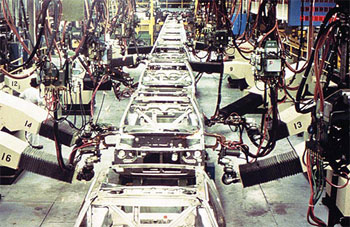
\includegraphics[scale=0.6]{img/unimate.jpg}
  		\caption{Unimate, General Motors}
  		\label{fig:unimate}
   	\end{minipage}\hfill
   	\begin {minipage}{0.48\textwidth}
     	\centering
     	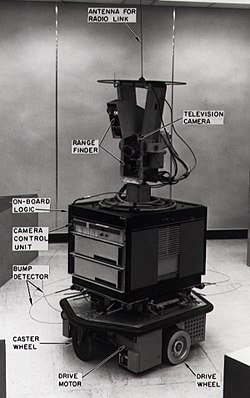
\includegraphics[scale=0.6]{img/shakey.jpg}
     	\caption{shakey en 1972}
     	\label{fig:shakey}
	\end{minipage}
\end{figure}

En 1970 se continua con la dinámica de crecimiento del sector, debido esta vez a la evolución del software ocurrida en esta época, y no parará hasta nuestros días, teniendo un crecimiento exponencial con una fuerte correlación con la evolución de software y hardware en general.
Desde este momento todas las grandes empresas dotaran sus fábricas de robots industriales. \\

En la actualidad uno de los mayores logros en el mundo de la robótica se da en 2011, la NASA lanzó al espacio el robot tipo vehículo explorador \textit{Curiosity} \ref{fig:curiosity} , que aterrizó en Marte al año siguiente. Su principal cometido es investigar la capacidad pasada y presente del planeta para alojar vida.\\

\begin{figure}[H]
    \centering
    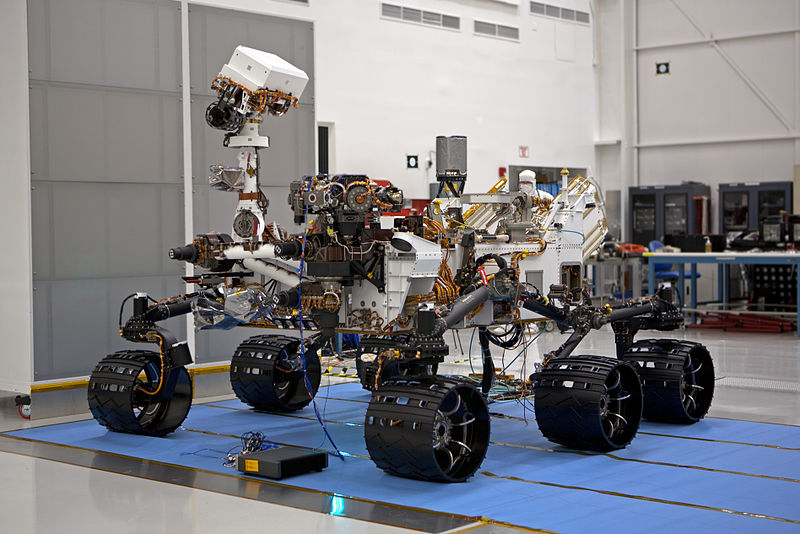
\includegraphics[scale=0.95]{img/curiosity.jpg}
  	\caption{El Curiosity en el Laboratorio de Propulsión a Chorro de la NASA}
  	\label{fig:curiosity}
\end{figure}

\subsection{Diferentes aplicaciones}
\label{subsec:diferentes aplicaciones}
Actualmente la robótica se encuentra en muchos ámbitos de nuestra vida cotidiana, algunas aplicaciones son:
\begin{itemize}
\item \textbf{Robótica educativa}: Es una disciplina que trabaja en la concepción creación e implementación de prototipos robóticos y programas con fines pedagógicos. Con ello se permite al alumno fabricar sus representaciones sobre los fenómenos del mundo, facilitar su adquisición y trasferencia a distintas áreas de conocimiento.
A través de la robótica educativa, los docentes pueden desarrollar de una forma práctica los conceptos teóricos que suelen ser abstractos y confusos, además despierta el interés del alumno por esos temas y relaciona al niño con el mundo tecnológico en el que se mueve. El empleo de un ambiente de aprendizaje basado en la robótica educativa ayuda al desarrollo de nuevas habilidades y conceptos, fortalece el pensamiento lógico, estructurado y formal del alumnado, desarrollando su capacidad para resolver problemas concretos.\\

Una de las características de este ámbito es la capacidad que posee para mantener la
atención del alumno, ya que manipula y experimenta haciendo que se concentre en sus
percepciones y observaciones sobre la actividad que realiza. Actualmente existen varios kits de robótica, algunos de ellos son: LEGO MINDSTORMS education, LEGO WeDo, LEGO NXT o Parallax Scribbler. Además, también existe la posibilidad de trabajar con programas con los que controlar y simular diferentes La robótica en Educación Infantil. Realidades y limitaciones robots como son NXT-G Educación, ROBOTC, ROBOLAB o Microsoft Robotics Developer Studio.

\item \textbf{Medicina}: Involucra en si varios ámbitos ya sea en cirugías de alto riesgo, en rehabilitaciones, en ayuda a personas con enfermedades de movilidad o discapacitados, en el almacenamiento de medicamentos y también en lo que se trata en pruebas ficticias y cirugías computarizadas.

\item \textbf{Militar}: La robótica donde más ha evolucionado es en la creación de vehículos autónomos, tecnología que tras unos años pasa a ser de uso civil.
Algunas de las creaciones que hemos heredado es el UAV, que se conocen comúnmente como dron, es una aeronave que vuela sin tripulación, Capaz de mantener de manera autónoma un nivel de vuelo controlado y sostenido, y propulsado por un motor de explosión, eléctrico, o de reacción.

\item \textbf{Robótica aeroespacial}: Uno de los mayores impulsores de la robótica ha sido la conquista del espacio, esta es una parte fundamental de la exploración espacial, debido a la imposibilidad de ser realizada en primera mano por un humano.
La idea básica sobre Robots Espaciales consiste en utilizar Inteligencia Artificial para
permitir a los robots realizar labores de exploración como si de un humano se tratase, desplazarse en terrenos y ambientes complejos de forma autónoma sin más conocimiento que lo recibido por sus sensores. Se busca no solo el proceso de pensamiento y análisis de los humanos en determinar las características del terreno, sino también la habilidad humana de conducir un vehículo en tiempo real.
\item \textbf{Industrial}: Las aplicaciones de la robótica industrial son cada vez mayores, algunos ejemplos son:
\begin{itemize}
\item Movimiento de material en almacenes: Un robot móvil es capaz de desplazarse por el almacén y recoger las unidades y referencias que incorporan un pedido concreto para un cliente.
\item Procesos de cadenas de montaje: Un robot antropomórfico es capaz de realizar movimientos complejos para colocar las distintas piezas que forman un producto final.
\item Empaquetado de producto: Tareas repetitivas y como puede ser el empaquetado de productos son realizadas por robots automatizados para hacer la misma tarea una y otra vez con alta velocidad y precisión, evitando errores y aumentando el ritmo de producción notablemente.
\item Procesos de alta precisión: Por ejemplo en la industria aeronáutica se utilizan cabezales de robots multifuncionales para el remachado en el fuselaje de un avión.
\item Seguimiento y verificación de productos: Un robot es capaz de realizar una evaluación al detalle del productor final, indicando si en el proceso de fabricación ha habido algún desperfecto o incorrección, estos robots suelen estar provistos de complejos sistemas de visión computacional.
\end{itemize}

\item \textbf{Automovilismo}: Los coches autónomos actualmente son una realidad, aún queda mucho desarrollo pero ya existen diversos modelos que se comercializan al público y conviven con el resto de automóviles. Esto es debido a la robustez que se ha conseguido en la lógica que gobierna estos coches. Se trata de uno de los retos cercanos más importantes de la robótica.\\
Para alcanzar una conducción realmente automática en una situación urbana con tráfico impredecible son necesarios muchos sistemas de tiempo real, que deben interoperar. Por ejemplo, es necesario un sistema de localización, de percepción del entorno, de planificación y lógicamente, un sistema de control. Además, son necesarios un conjunto de sensores que recojan y proporcionen la información necesaria para poder tomar las decisiones.

\item \textbf{Domótica}: Es el conjunto de tecnologías aplicadas al control y la automatización inteligente de la vivienda, que permite una gestión eficiente del uso de la energía, que aporta seguridad y confort, además de comunicación directa con los diferentes sistemas y elementos de una casa a través de la red.

Un sistema domótico es capaz de recoger información proveniente de unos sensores o entradas, procesarla y emitir órdenes a unos actuadores o salidas. El sistema puede acceder a redes exteriores de comunicación o información.
\end{itemize}

Es difícil no parase a pensar en la potencia que tiene esta rama de la ciencia y la
tecnología. Todo lo comentado deja claro la utilidad de esta área de desarrollo, que permitirá en el futuro ganar en comodidad, economía e incluso salud.

\subsection{Tipos de Robots}
\label{subsec:tipos de robots}

Ningún autor se pone de acuerdo en cuántos y cuáles son los tipos de robots y sus características esenciales. La más común son la que a continuación se presentan:

\textbf{Según su Estructura}:
\begin{itemize}
\item \textbf{Androides}: Un robot humanoide que se limita a imitar los actos y gestos de un humano, no es visto por el público como un verdadero androide, sino como una simple marioneta controlada por un humano. El androide siempre ha sido representado como una entidad que imita al ser humano tanto en apariencia, como en capacidad mental e iniciativa

\item \textbf{Poliarticulados}: En este grupo pueden encontrarse robots de diversas formas y configuraciones, pero su característica en común es la de ser sedentarios. Es decir, que son robots estructurados para moverse en un determinado espacio de trabajo, según uno o más sistemas de coordenadas y con un número limitado de grados de libertad.

\item \textbf{Móviles}: Estos robots cuentan con orugas, ruedas o patas que les permiten desplazarse de acuerdo a la programación a la que fueron sometidos. Estos robots cuentan con sistemas de sensores, que son los que captan la información que dichos robots elaboran. Los móviles son utilizados en instalaciones industriales, en la mayoría de los casos para transportar la mercadería en cadenas de producción así como también en almacenes. Además, son herramientas muy útiles para investigar zonas muy distantes o difíciles de acceder, es por eso que se suelen utilizar para realizar exploraciones espaciales o submarinas.

\item \textbf{Zoomórficos}: La locomoción de estos robots imita a la de distintos animales y se los puede dividir en caminadores y no caminadores. Estos últimos están aún muy poco desarrollados mientras que los caminadores sí lo están y resultan útiles para la exploración volcánica y espacial.

\item \textbf{Híbridos}: Este término corresponde a todos aquellos robots que son difíciles de clasificar, ya que corresponden a una combinación de las estructuras anteriormente explicadas. Por ejemplo, un robot híbrido, que esté conformado por la segmentación de articulaciones y ruedas, podría ser considerado tanto móvil, así como zoomórfico.

\end{itemize}

\begin{figure}[H]
	\begin{minipage}{0.48\textwidth}
    	\centering
     	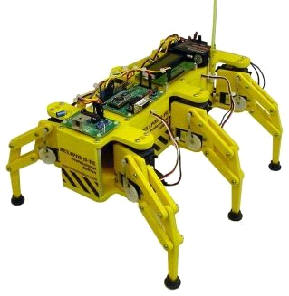
\includegraphics[scale=0.6]{img/robot-zoomorfico.jpg}
  		\caption{Robot zoomórfico}
  		\label{fig:zoomorfico}
   	\end{minipage}\hfill
   	\begin {minipage}{0.48\textwidth}
     	\centering
     	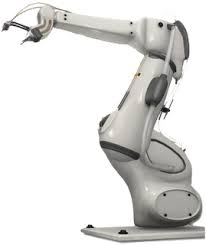
\includegraphics[scale=0.6]{img/robot-poliarticulado.jpg}
     	\caption{Robot poliarticulado}
     	\label{fig:poliarticulado}
	\end{minipage}
\end{figure}


\textbf{Según su Cronología}:
\begin{itemize}
\item \textbf{1ª Generación. Manipuladores}: Son sistemas mecánicos multifuncionales con un sencillo sistema de control, bien manual, de secuencia fija o de secuencia variable.

\item \textbf{2ª Generación. Robots de aprendizaje}: Repiten una secuencia de movimientos de movimientos que ha sido ejecutada previamente por un operador humano. El modo de hacerlo es a través de un dispositivo mecánico. El operador realiza los movimientos requeridos mientras el robot le sigue y los memoriza.

\item \textbf{3ª Generación. Robots con control sensorizado}: El controlador es una computadora que ejecuta las órdenes de un programa y las envía al manipulador para que realice los movimientos necesarios.

\item \textbf{4ª Generación. Robots inteligentes}: Son similares a los anteriores, pero además poseen sensores que envían información a la computadora de control sobre el estado del proceso. Esto permite una toma inteligente de decisiones y el control del proceso en tiempo real.
\end{itemize} 


\section{Software para robots}

Muchos robots poseen autonomía, la cual proviene del desarrollo de sistemas complejos, aplicaciones e infraestructuras que les dotan de inteligencia autónoma. El desarrollo de software robótico es similar al desarrollo de software en otros ámbitos, donde se parte de ciertos requisitos y se modela un diseño que será creado. Hace años el desarrollo de software robótico se realizaba adoptando soluciones ``ad hoc'', dotando a cada robot de un diseño específico, y con sensores y actuadores concretos. Esto suponía que no se podía aplicar el software desarrollado a otro robot, por lo que era necesario implementar de nuevo todo el software para un nuevo robot. En la actualidad, existen numerosas plataformas que permiten el desarrollo de aplicaciones robóticas de forma eficiente y genérica. Esto permite reutilizar gran parte de las aplicaciones creadas en otros robots, evitando el coste de realizar todo el proceso de nuevo.\\

Dotar al robot de cierta inteligencia conlleva desarrollar cierto software, el cual se suele programar apoyándose en herramientas, como los middleware robóticos, los simuladores robóticos, o las  bibliotecas que facilitan algunos aspectos. A continuación, se exponen algunas de estas herramientas que se emplean en la actualidad.\\

\subsection{Middlewares robóticos}

Actualmente existen diversos middlewares robóticos, con los que somos capaces de gestionar la complejidad y heterogeneidad del hardware y las aplicaciones, promover la integración de tecnologías en desarrollo, enmascarar los sistemas de percepción complejos, y simplificar el diseño de software.\\

Mediante el uso de middlewares somos capaces de introducir una capa de abstracción con los drivers y el hardware del robot, disminuyendo de manera importante la complejidad y los conocimientos necesarios para cualquier desarrollo. Además permite paralelizar de forma eficiente el trabajo.\\

\begin{figure}[H]
    	\centering
     	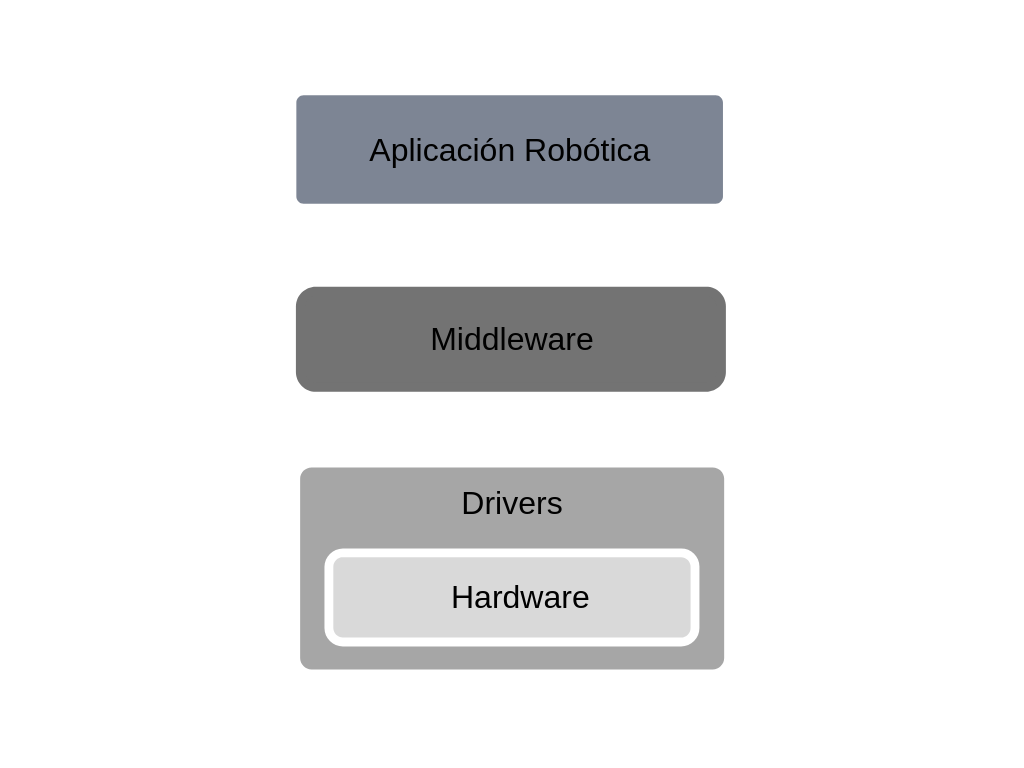
\includegraphics[scale=0.40]{img/middleware.png}
  		\caption{Esquema de capas en desarrollos de aplicaciones robóticas}
  		\label{fig:middleware}
\end{figure}

Algunos de los middlewares robóticos más destacados son:

\begin{itemize}
\item \textbf{ROS}\footnote{\url{http://www.ros.org/}}: Es una plataforma de software libre para el desarrollo de software de robots, que provee servicios estándar de un sistema operativo como la abstracción del hardware, el control de dispositivos de bajo nivel, mecanismos de intercambio de mensajes entre procesos y un conjunto de herramientas utilizadas ampliamente en robótica. La librería está orientada para un sistema UNIX, aunque se está adaptando a otros sistemas operativos como Fedora, Mac OS X, Arch, Gentoo, OpenSUSE, Slackware, Debian o Microsoft Windows, considerados como ``experimentales''.
En futuros capítulos hablaremos más en profundidad sobre ROS y su funcionamiento.
\item \textbf{Orocos}\footnote{\url{http://www.orocos.org}}: Es un proyecto de software libre para el control de robots y máquinas. Incluye cuatro bibliotecas C++: Real-Time Toolkit, Kinematics and Dynamics Library,  Bayesian Filtering Library y  Orocos Component Library. Está orientado a componentes, permitiendo añadir funcionalidades de forma sencilla y sin recompilar todo el código.  Incluye paquetes complementarios tales como Filtros de Bayes, Librerías de control Dinámico y Cinemático o Visión.

\item \textbf{Orca}\footnote{\url{http://orca-robotics.sourceforge.net/}}: Se trata de una plataforma de software libre para el desarrollo de aplicaciones robóticas. Fundamentalmente orientada al desarrollo de componentes, proporciona los medios para definir y desarrollar los componentes, los cuales pueden unirse para formar sistemas robóticos de distintas complejidades, desde vehículos autónomos hasta redes de sensores distribuidas.
Orca permite reutilizar código, de manera que se pueden emplear componentes robóticos ya creados.
\end{itemize}

\subsection{Simuladores robóticos}
El diseño de un robot es costoso y caro, lo que implica que muchos componentes necesarios para la construcción de los robots solamente estén disponibles para centros de investigación y corporaciones. Cuando se emplea un robot puede que el código desarrollado falle al probarlo, pudiendo incluso romperse algún robot.\\

Hoy en día existen numerosos simuladores robóticos, lo que permite a cualquier persona crear, programar y probar infinidad de robots de forma segura y económica. Algunos de los simuladores más empleados son:

\begin{itemize}
\item \textbf{Gazebo}\footnote{\url{http://gazebosim.org/}}: Es un simulador 3D de código abierto distribuido bajo licencia Apache 2.0. Este simulador se ha utilizado en ámbitos de investigación en robótica e Inteligencia Artificial. Contiene un potente motor de renderizado, soporta la incorporación de plugins lo que le hace ganar versatilidad, por ejemplo para integrarse middleware como ROS. Al ser muy popular y tener una gran comunidad se puede encontrar un amplio repertorio de robots comerciales.
\item \textbf{Stage}\footnote{\href{http://playerstage.sourceforge.net/index.php?src=stage}{stage}}: Simula robots móviles en el plano bidimensional y proporciona diversos tipos de sensores y actuadores. Su finalidad es ayudar a la investigación de sistemas autónomos de múltiples agentes, para lo cual proporciona gran cantidad de dispositivos simultáneamente.
\item \textbf{Webots}\footnote{\url{https://cyberbotics.com/}}: Es un simulador avanzado de robótica, que permite definir modelos propios, definir la física, escribir controladores para los robots y hacer simulaciones a gran velocidad. Se puede emplear en los sistemas operativos Linux, Windows y MacOS. Los lenguajes de programación que se pueden emplear son  C++, C y Java.
\end{itemize}

\subsection{Bibliotecas}
Las bibliotecas referidas al contexto de software son un conjunto de desarrollos que pueden ser usadas por terceros mediante una serie de interfaces bien definidas, que aportan de una funcionalidad añadida evitando tener que ser desarrollada desde un cero por el desarrollador que hace uso de ellas. Esto hace que agilicen y ayuden de forma notable cualquier proyecto, ya que únicamente debes centrarte en lo relativo a tu lógica, mientras que las cosas comunes puedes integrarlas en tu código a través de estas librerías.\\

Algunas de las bibliotecas utilizadas en robótica son:

\begin{itemize}
\item \textbf{OpenCV}\footnote{\url{https://opencv.org/}}: Es una biblioteca orientada principalmente a la visión computacional en tiempo real. La biblioteca es multiplataforma y gratuita para su uso bajo la licencia BSD de código abierto. Entre las áreas de aplicación de esta biblioteca destacan: segmentación y reconocimiento de objetos, reconocimiento de gestos, seguimiento del movimiento, estructura del movimiento,  y robots móviles.
\item \textbf{PCL}\footnote{\url{http://pointclouds.org/}}: Se utiliza para el procesamiento digital de imágenes RGBD mediante el tratamiento de nubes de puntos 3D. Contiene numerosos algoritmos de última generación que incluyen filtrado, estimación de características, reconstrucción de superficies, ajuste de modelos y segmentación entre otros. Para simplificar el desarrollo, PCL se divide en una serie de bibliotecas de código más pequeñas, que se pueden compilar por separado. Es multiplataforma y ha sido compilada con éxito en Linux, Mac OSX, Windows y Android / iOS
\item \textbf{AForge.NET}\footnote{\url{http://www.aforgenet.com/}}: Es un framework C\# de código abierto diseñado para desarrolladores e investigadores en los campos de Visión por Computadora e Inteligencia Artificial. Sus áreas de aplicación son: procesamiento de imágenes, redes neuronales, algoritmos genéticos, lógica difusa, aprendizaje de máquinas, robótica, etc.
\end{itemize}

\section{Docencia en robótica}

Actualmente la robótica es un mercado al alza, esto hace que aumente de manera importante el número de científicos, ingenieros y técnicos demandados para trabajar e investigar en este sector.
Es importante una base sólida en conceptos de programación, procesado de imágenes, calculo, álgebra, electrónica, electricidad etc. Al ser un mundo complejo lleno de retos por resolver se necesita gente preparada, de ahí lo importante que es acercar a los más jóvenes desde los colegios e institutos a estas disciplinas.\\

Es por esto que la docencia en robótica intenta despertar el interés de los estudiantes transformando las asignaturas tradicionales en más atractivas e integradoras, ya que crea entornos de aprendizaje propicios que recrean los problemas del entorno que los rodea. En el futuro, tener nociones básicas de esta disciplina será clave debido a que cada vez de forma más habitual se implantan robots en diferentes sectores laborales.\\

La enseñanza en centros escolares principalmente se realiza mediante plataformas físicas como los robots LEGO (Mindstorms, NXT, Evo, WeDo), placas Arduino, los kits de SolidWorks, etc que con una simpleza espectacular son capaces de motivar al alumno ya que obtiene resultados vistosos y a los que le puede dar una aplicación en su vida cotidiana, despertando su interés en esta materia.\\
Otro sistema introducido en los últimos años en la educación es la programación de robots mediante lenguajes de programación visual, potentes lenguajes, que abstrayendo al alumno de la complejidad de la sintaxis, siendo muy intuitivos y dándole un entorno visual vistoso, hacen que estos software sean muy bien aceptados por los estudiantes de menor edad.\\

La capacidad de programar es una parte importante de la alfabetización en la sociedad actual. Cuando las personas aprenden a programar, aprenden estrategias importantes para resolver problemas, diseñar proyectos y comunicar ideas.

\section{Lenguajes de programación visual}
\label{sec:lenguajes}

Un lenguaje de programación visual es cualquier lenguaje de programación que permite a los usuarios crear programas manipulando elementos del programa gráficamente en lugar de especificarlos textualmente. Permite la programación con expresiones visuales y símbolos gráficos, utilizados como elementos de sintaxis o notación secundaria. Por ejemplo, muchos se basan en la idea de "cajas y flechas", donde las cajas u otros objetos de pantalla se tratan como entidades, conectadas por flechas, líneas o arcos que representan relaciones, mientras que otros se basan en el apilamiento de "cajas" con una función predefinida, creando así varios flujos de acciones programáticas con una objetivo final.\\

Estos lenguajes por regla general se usan en programación dirigida por eventos, La programación dirigida por eventos es un paradigma de programación en el que el flujo del programa está determinado por eventos o mensajes desde otros programas o hilos de ejecución.
Las aplicaciones desarrolladas con programación dirigida por eventos implementan un bucle principal o main loop donde se ejecutan las dos secciones principales de la aplicación: El selector de eventos y el manejador de eventos.\\

Podemos diferenciar varios niveles dentro de los lenguajes de programación visual:
\begin{itemize}
\item \textbf{Sintaxis}: En el nivel sintáctico, la explicación del bloque está limitada a estructura del lenguaje. Por ejemplo, una explicación podría revelar que una condición es parte de una declaración \textit{IF} y no debe ser confundido con una acción que se puede ejecutar en \textit{THEN} o \textit{ELSE} parte de una declaración. Sin embargo, este no trata de definir de forma específica qué es lo que define esa condición.
Intentan reducir o incluso eliminar por completo los errores sintácticos y ayudan a la creación de programas bien formados. Una analogía sería el corrector ortográfico en procesadores de texto que subraya o incluso corrige automáticamente palabras o gramática individuales.

\item \textbf{Semántica}: En el nivel de la semántica, se dan explicaciones sobre los bloques, a menudo implementadas a través de funciones de ayuda que describen el significado
de un bloque. El usuario obtiene una respuesta semántica en forma de panel de ayuda genérico incluyendo una breve descripción del significado del comando o bloque y la lista de opciones adicionales.

\item \textbf{Pragmática}: Permiten llevar nuestra implementación a un punto de testeo específico, nos ayudan con una serie de módulos propios a crear el entorno necesario para simular el funcionamiento de nuestro programa en ese estado.
\end{itemize}

\subsection{Motivación}
\label{subsec:motivacion}

Las principales motivaciones del uso de estos lenguajes son su \textbf{accesibilidad}, ya que no requiere de una infraestructura potente para su funcionamiento.
Además el \textbf{fácil aprendizaje} hace que sea un lenguaje idóneo para aquellos que no tienen ningún conocimiento de informática previo.
Y por último el eliminar de la ecuación algo tan simple como los \textbf{errores de sintaxis}, nos olvidamos completamente de este tipo de fallos, haciendo el desarrollo más fluido y menos frustrante para los principiantes, algo que puede marcar la diferencia a la hora de encontrar gratificante el desarrollo de aplicaciones con estos lenguajes.

\subsection{Ejemplos}
\label{subsec:tipos}

\begin{itemize}

\item \textbf{Scratch}\footnote{\url{https://scratch.mit.edu/}}: Es un proyecto del Grupo Lifelong Kindergarten del MIT Media Lab.
Es utilizado por estudiantes y docentes de todo el mundo para expresar ideas mediante animaciones, juegos e interacciones fácilmente programables con este entorno, hablaremos en capítulos siguientes más en profundidad de él.

\item \textbf{Blocly}\footnote{\url{https://developers.google.com/blockly/}}: El desarrollo de Blockly comenzó en el verano de 2011, y el primer lanzamiento público fue en Maker Faire en mayo de 2012. Blockly fue originalmente diseñado como un reemplazo para OpenBlocks en App Inventor. Es un proyecto de Google y es de código abierto. Por lo general, se ejecuta en un navegador web y se asemeja visualmente a Scratch. Blockly también se está implementando para Android e iOS aunque no todas las funciones basadas en el navegador web están disponibles para Android / iOS.
Utiliza bloques visuales que se unen entre sí para facilitar la escritura de códigos y generar código JavaScript, Python, PHP o Dart.

\begin{figure}[H]
    \centering
    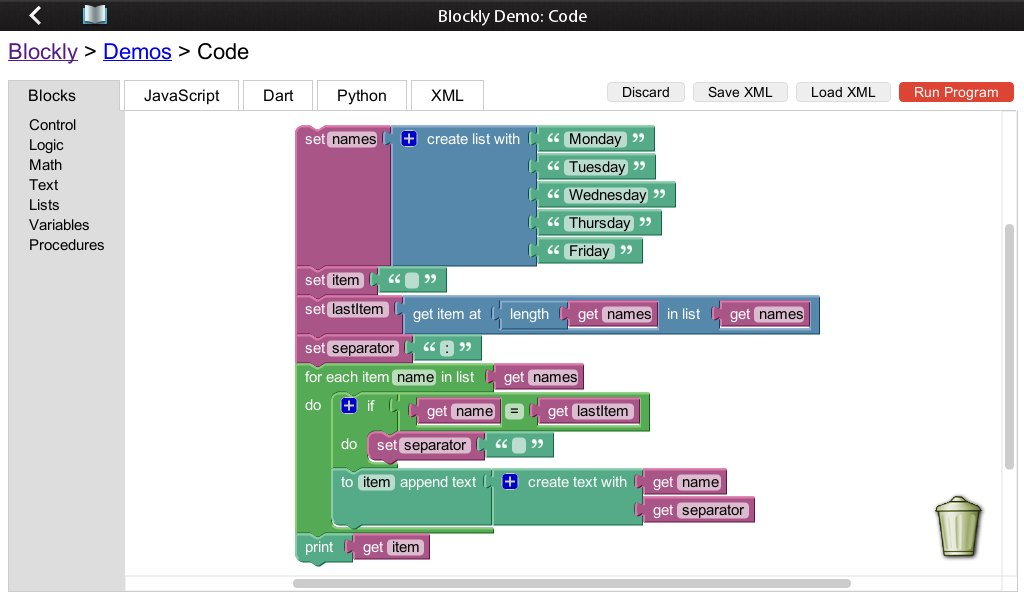
\includegraphics[scale=0.40]{img/blockly.jpg}
  	\caption{Lenguaje de programación visual Blockly}
  	\label{fig:blockly}
\end{figure}

\item \textbf{Snap!}\footnote{\url{https://snap.berkeley.edu/}}: Desarrollada por la Universidad de California en Berkeley, que sigue la filosofía de facilidad y sencillez para aprender a programar, Snap se basa en el conocido programa de Scratch, siendo su uso más extendido entre edades más maduras que las de Scratch.
Snap está programado en JavaScript. Esto hace que podamos usarlo desde cualquier navegador, ya sea desde un ordenador como desde las tablets.

\begin{figure}[H]
\centering
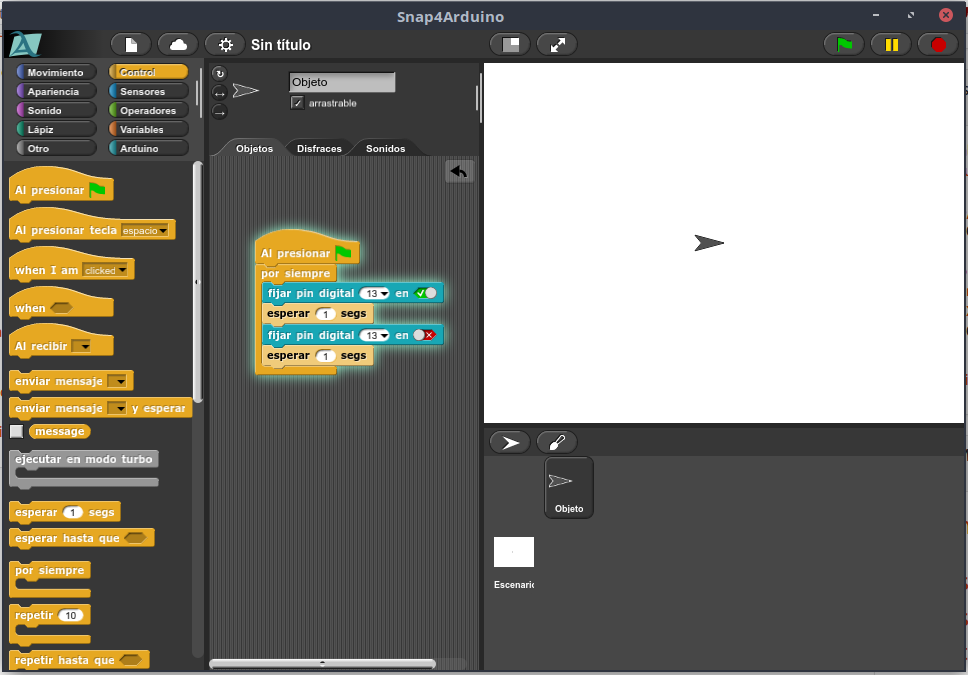
\includegraphics[scale=0.40]{img/snap.png}
\caption{Lenguaje de programación visual Snap!}
\label{fig:snap}
\end{figure}

\item \textbf{Kodu}\footnote{\url{https://www.kodugamelab.com/}}: Originalmente llamado Boku, es un entorno de desarrollo integrado de programación (IDE) de los laboratorios FUSE de Microsoft. El modelo de programación de Kodu está simplificado y puede programarse utilizando un controlador de juegos. Prescinde de la mayoría de las convenciones de programación que incluyen variables simbólicas, bucles, manipulación de números y cadenas, subrutinas, polimorfismo, etc.

Esta simplicidad se logra al ubicar la tarea de programación en un entorno de simulación ampliamente completo. El usuario programa los comportamientos de los personajes en un mundo 3d, y los programas se expresan en un paradigma sensorial de alto nivel que consiste en un sistema o lenguaje basado en reglas, basado en condiciones y acciones.

\begin{figure}[H]
\centering
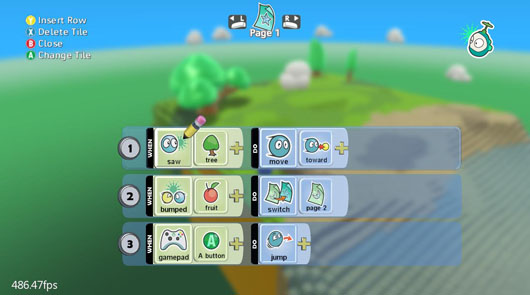
\includegraphics[scale=1]{img/kodu.jpg}
\caption{Lenguaje de programación visual Kodu}
\label{fig:kodu}
\end{figure}

\item \textbf{LEGO}: Lego dispone de una amplia gama de robots de aprendizaje programables (Mindstorms, NXT, Evo, WeDo), cada uno de estos robots de aprendijaze posee su propia sistema de programación, todos bajo interfaces gráficas fácilmente manipulables e intuitivas.\\
\begin{figure}[H]
	\begin{minipage}{0.48\textwidth}
    	\centering
     	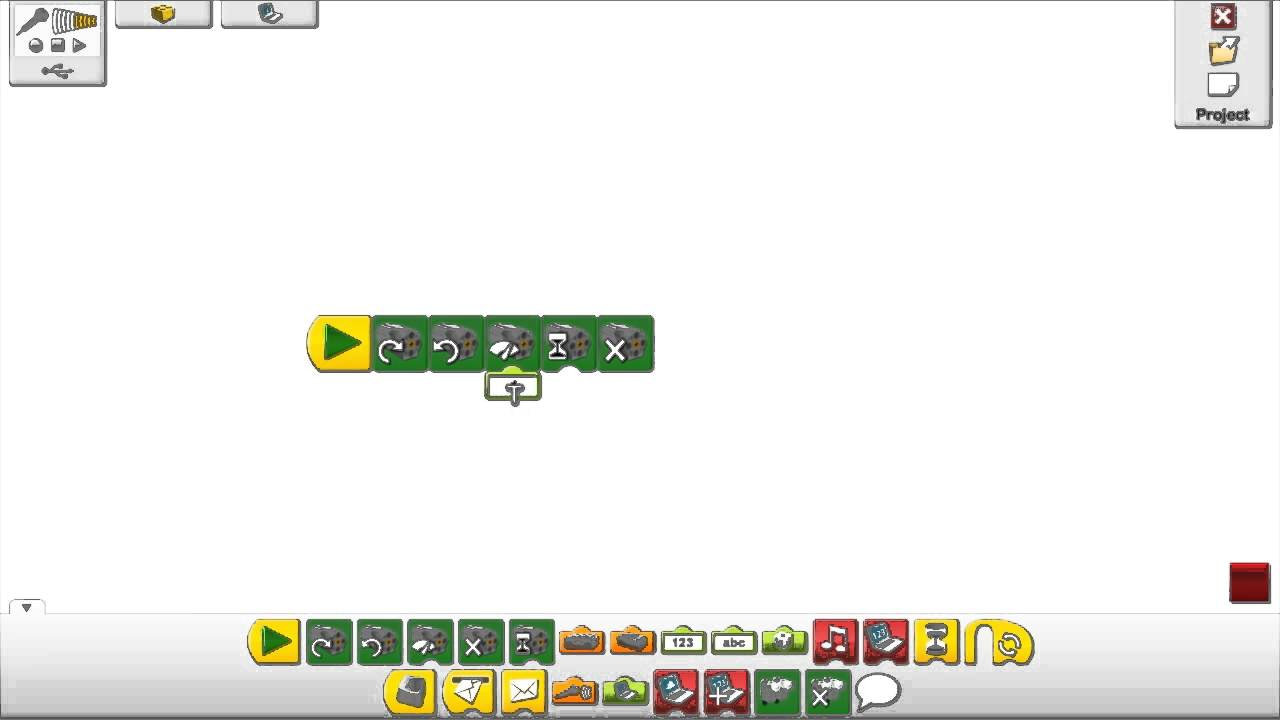
\includegraphics[scale=0.15]{img/lego-wedo.jpg}
  		\caption{Software de programación visual para LEGO WeDo}
  		\label{fig:lego-wedo}
   	\end{minipage}\hfill
   	\begin {minipage}{0.48\textwidth}
     	\centering
     	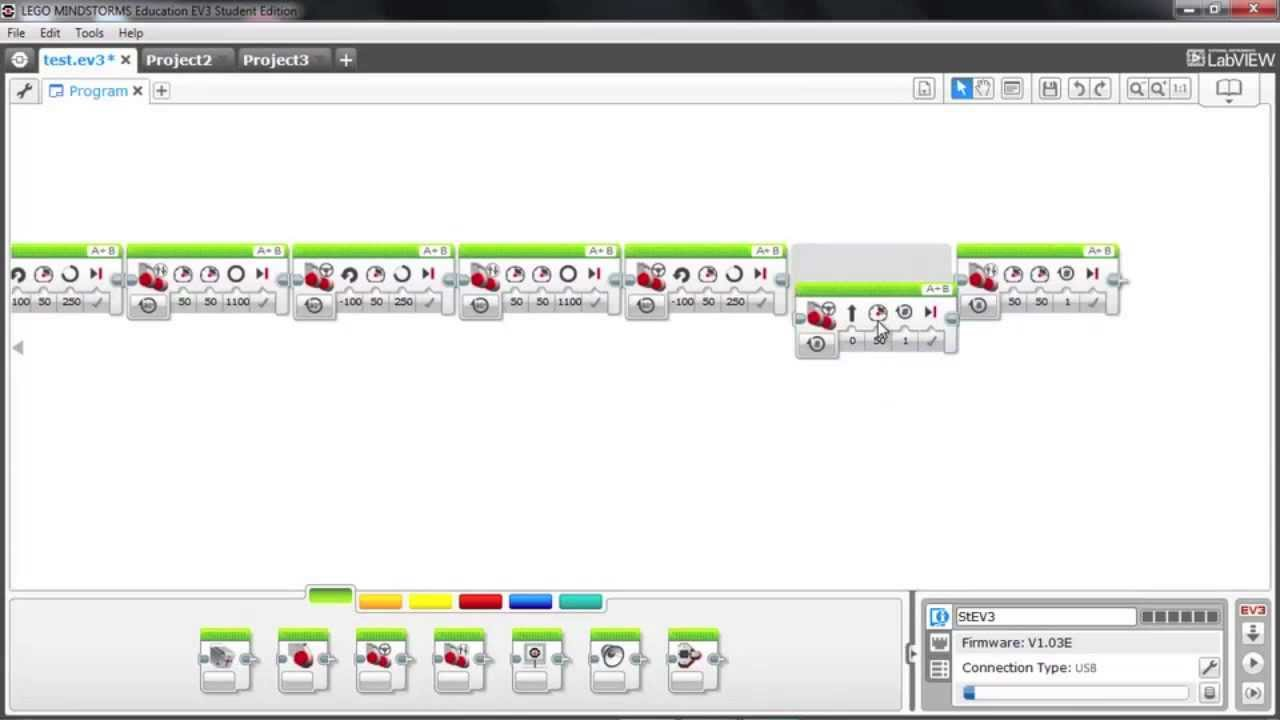
\includegraphics[scale=0.15]{img/lego-mindstorms.jpg}
     	\caption{Software de programación visual para LEGO Mindstroms}
     	\label{fig:lego-mindstorms}
	\end{minipage}
\end{figure}

\item \textbf{VisualStates}\footnote{\url{http://jderobot.org/VisualStates}}: Herramienta integrada en la suit de programación JdeRobot es una herramienta para la programación de comportamientos de robot utilizando máquinas de estados finitos de jerarquía (HFSM - Hierarchichal Finite State Machine). Representa gráficamente el comportamiento del robot en un esquema compuesto por estados y transiciones. Cuando el autómata está en cierto estado, pasará de un estado a otro según las condiciones establecidas en las transiciones. Esta representación gráfica permite un mayor nivel de abstracción para el usuario, ya que solo tiene que preocuparse por programar las acciones del robot y seleccionar qué componentes puede necesitar de la interfaz del robot.\\


\begin{figure}[H]
\centering
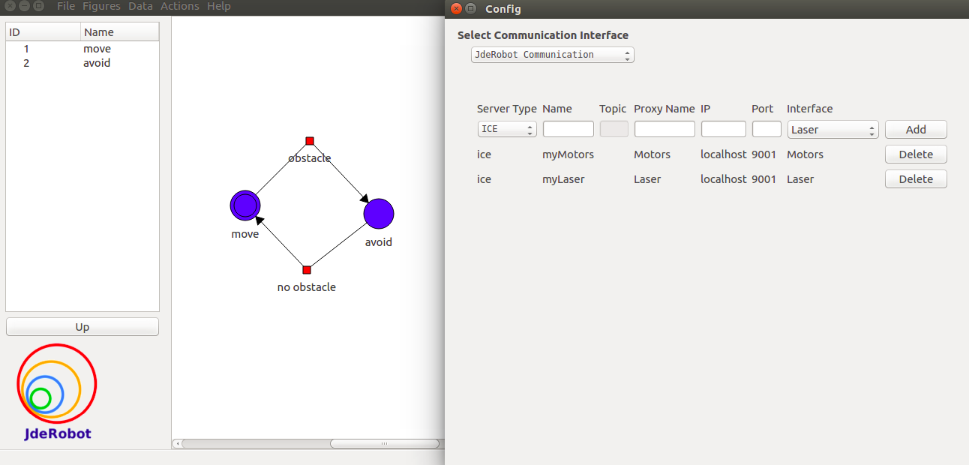
\includegraphics[scale=0.40]{img/visualstates.png}
\caption{Lenguaje de programación visual VisualStates}
\label{fig:visualstates}
\end{figure}

\item \textbf{Choregraphe}: Es el software de programación que permite a los usuarios crear y editar movimientos y comportamientos de NAO de manera sencilla. Su intuitiva interfaz gráfica, su biblioteca de comportamientos y las funciones de programación hacen posible realizar desde tareas simples como de nivel avanzado.

Es posible crear comportamientos utilizando la biblioteca de bloques de comportamiento con un simple arrastrar/copiar.
permite la programación basada en eventos, secuencial o en paralelo. Además la línea de tiempo permite programar por medio de secuencia lógica.

Los bloques de comportamiento pre-programadas son fácilmente configurables y con el editor de curvas o por medio de lenguaje Python.\\


\end{itemize}